%%%%%%%%%%%%%%%%%%%%%%%%%%%%%%%%%%%%%%%%%%%%%%%%%%%%%%%
% A template for Wiley article submissions developed by 
% Overleaf for the Overleaf-Wiley pilot which ran 
% during 2017 and 2018.
% 
% This template is no longer supported, but is provided
% for historical reference. Last updated January 2019.
%
% Please note that whilst this template provides a 
% preview of the typeset manuscript for submission, it 
% will not necessarily be the final publication layout.
%
% Document class options:
% =======================
% blind: Anonymise all author, affiliation, correspondence
%        and funding information.
%
% lineno: Adds line numbers.
%
% serif: Sets the body font to be serif. 
%
% twocolumn: Sets the body text in two-column layout. 
% 
% num-refs: Uses numerical citation and references style 
%           (Vancouver-authoryear).
%
% alpha-refs: Uses author-year citation and references style
%             (rss).
%
% Using other bibliography styles:
% =======================
%
% To specify a different bibiography style
%
% 1) Do not use either num-refs or alpha-refs in documentclass.
% 2) Load natbib package with the options set as needed.
% 3) Use the \bibliographystyle command to specify the style
% 
% Included NJD styles are: 
%   WileyNJD-ACS
%   WileyNJD-AMA
%   WileyNJD-AMS
%   WileyNJD-APA
%   WileyNJD-Harvard
%   WileyNJD-VANCOUVER
%
% or you may upload an alternative .bst file 
% (if requested by the journal).
%
% Examples:
% =======================
%% Example: Using numerical, sort-by-authors citations.
\documentclass[num-refs, serif]{wiley-article}

%% Example: Using author-year citations and anonymising submission
% \documentclass[blind,alpha-refs]{wiley-article}

%% Example: Using unsrtnat for numerical, in-sequence citations
% \documentclass{wiley-article}
% \usepackage[numbers]{natbib}
% \bibliographystyle{unsrtnat}

%% Example: Using WileyNJD-AMA reference style and superscript
%%          citations, two-column and serif fonts for AIChE
% \documentclass[serif,twocolumn,lineno]{wiley-article}
% \usepackage[super]{natbib}
% \bibliographystyle{WileyNJD-AMA}
% \makeatletter
% \renewcommand{\@biblabel}[1]{#1.}
% \makeatother

% Add additional packages here if required
\usepackage{siunitx}
\usepackage{booktabs}
\usepackage{adjustbox}
\usepackage[textsize=footnotesize]{todonotes}

% Update article type if known
\papertype{FHNW Paper}

\title{Perfomancevergleich von Zigbee, Thread und Bluetooth Mesh Netzwerken}

% List abbreviations here, if any. Please note that it is preferred that abbreviations be defined at the first instance they appear in the text, rather than creating an abbreviations list.
\abbrevs{ABC, a black cat; DEF, doesn't ever fret; GHI, goes home immediately.}

% Include full author names and degrees, when required by the journal.
% Use the \authfn to add symbols for additional footnotes and present addresses, if any. Usually start with 1 for notes about author contributions; then continuing with 2 etc if any author has a different present address.
\author[1]{Cyrill Horath}
\author[1]{Raffael Anklin}
\author[1]{Robin Bobst}

% Include full affiliation details for all authors
\affil[1]{Institut für ??, Fachhochschule Nordwestschweiz, Windisch, Aargau, 5210, Schweiz}

\corraddress{Team Blau, Institut für ??, Fachhochschule Nordwestschweiz, Windisch, Aargau, 5210, Schweiz}
\corremail{TeamBlau@email.com}

%\presentadd[\authfn{2}]{Department, Institution, City, State or Province, Postal Code, Country}

%\fundinginfo{Funder One, Funder One Department, Grant/Award Number: 123456, 123457 and 123458; Funder Two, Funder Two Department, Grant/Award Number: 123459}

% Include the name of the author that should appear in the running header
\runningauthor{Perfomancevergleich Zigbee, Thread, Bluetooth}

\begin{document}
\begin{figure}
	
\includegraphics[scale=1]{graphics/fhnw_ht_logo_de.pdf}
\end{figure}

\begin{frontmatter}
\maketitle

% Document abstract:
% ==========================================
\begin{abstract}
\todo[inline]{Abstract hinzufügen}

% Please include a maximum of seven keywords
\keywords{keyword 1, \emph{keyword 2}, keyword 3, keyword 4, keyword 5, keyword 6, keyword 7}
\end{abstract}
\end{frontmatter}

% Document sections:
% ==========================================

\newpage
\section{Einleitung}
\todo[inline]{In der Einleitung sollen die drei verschiedenen Stacks kurz und knapp erläutert werden und welche Vor- und Nachteile diese haben.}
Im 2.4GHz ISM-Band kon­kur­ren­zie­ren sich derzeit die drei weit verbreiteten Low Power Mesh Netzwerk Protokolle Bluetooth Mesh, Thread und Zigbee.
Alle drei wurden konzipiert für die kabellose Übertragung in sogenannten WSN (Wireless Sensor Networks) oder in Netzen für die Heim Automatisierung. Während Thread und Zigbee den IEEE 802.15.4 Standard als Physical Layer benutzen basiert der BT Mesh Stack auf dem BLE (Bluetooth Low Energy) Standard. Aufgrund der hohen Dichte an Netzwerkprotokollen die das 2.4GHz ISM-Band ebenso nutzen (z.B. Wifi) sind die Störeinflüsse auf die Mesh Protokolle eines der grössten Probleme. Die Protokollstacks begegnen diesem und weiteren Problemen auf unterschiedliche Weise. Diese Unterschiede und schliesslich die Performance der Mesh Netzwerke sollen unter unterschiedlichen Testbedingungen aufgezeigt werden wodurch ein objektiver Vergleich der drei Mesh Protokolle möglich wird.

\begin{table}[h]
	\centering
	\begin{adjustbox}{width=1\textwidth}
	\begin{tabular}{@{}|l|l|l|l|@{}}
		\toprule
		\multicolumn{4}{|c|}{\textbf{Mesh Netzwerke im Vergleich}}                                                                                                            \\ \midrule
		& \textbf{Bluetooth Mesh}              & \textbf{Thread}                                  & \textbf{ZigBee}                              \\ \midrule
		\textbf{Markt}               & Beleuchtung und Smart Home           & Industrie und Smart Home                         & Beleuchtung, Haus Automation und Messtechnik \\ \midrule
		\textbf{Veröffentlicht}      & 2017                                 & 2015                                             & 2003                                         \\ \midrule
		\textbf{Appllikations Layer} & Mesh Model System                    & Verknüfpbar mit allen IPv6 basierten Protokollen & Cluster Bibliothek                           \\ \midrule
		\textbf{IPv6}                & Nein                                 & Ja                                               & Nein                                         \\ \midrule
		\textbf{Netzwerk Zugriff}    & Smartphone oder Gateway              & Border Router                                    & Gateway                                      \\ \midrule
		\textbf{Ökosysteme}          & Ledvance                             & Google Nest                                      & Ikea, Phillips Hue, Amazon und weitere       \\ \midrule
		\textbf{Routing}             & Managed Flooding                     & Geroutet                                         & Geroutet                                     \\ \midrule
		\textbf{Weiteres}            & Ist direkt mit Smartphone erreichbar & Automatisiertes Verwalten des Netzwerks          & Am meisten verbreitet                        \\ \bottomrule
	\end{tabular}
	\end{adjustbox}
	\caption{Vergleich Mesh Netzwerke}
	\label{table:VergleichMeshNetzwerk}
\end{table}

\section{Methode}
Um die Performance der drei Mesh Stacks zu vergleichen wurde ein einheitliches Benchmark Konzept erarbeitet. Dieses definiert die Mesh Parameter, Testumgebungen, den Ablauf sowie sämtliche Messgrössen und Messreihen.

\subsection{Messablauf}
Für den Vergleich der 3 Mesh Netzwerkstacks Bluetooth Mesh (BT Mesh), Thread und Zigbee wird ein vom Mesh Protokoll unabhängiges Testkonzept umgesetzt welches in der Abbildung \ref{fig:KonzeptschemaTestablauf} als Konzeptschema dargestellt ist. Die Benchmark Slave Nodes (BSN) in der Abbildung als Sensoren und Aktoren mit unterschiedlichen Funktionalitäten dargestellt, bilden zusammen mit dem Benchmark Master Node (BMN) das zu testende Mesh Netzwerk. Innerhalb des Netzwerks wird dessen Organisation vom jeweiligen Protokoll sichergestellt. Das Testnetzwerk soll ein realitätsnahes Netzwerk nachbilden. Beispielsweise wird eine Hausautomation in einem Einfamilienhaus als Referenz angenommen in welchem jeweils nur gewisse Nodes untereinander Applikationsdaten austauschen. Ein Lichtschalter kommuniziert nur mit einer Lichtquelle und umgekehrt. Der selbe Lichtschalter tauscht jedoch keine Applikationsdaten mit dem Temperatursensor aus. Trotzdem bilden die Nodes zusammen ein Mesh Netzwerk.\\

Die Benchmark Management Station (BMS) welche mit dem BMN via USB/UART kommuniziert, ist zuständig für die Verwaltung und Verarbeitung der Benchmarks. Während eines Benchmark Prozesses sollen sämtliche Messungen jedoch unabhängig von der BMS durchgeführt werden damit allfällige Latenzzeiten der USB/UART Verbindung die Resultate nicht verfälschen.

\begin{figure}[h]
	\centering
	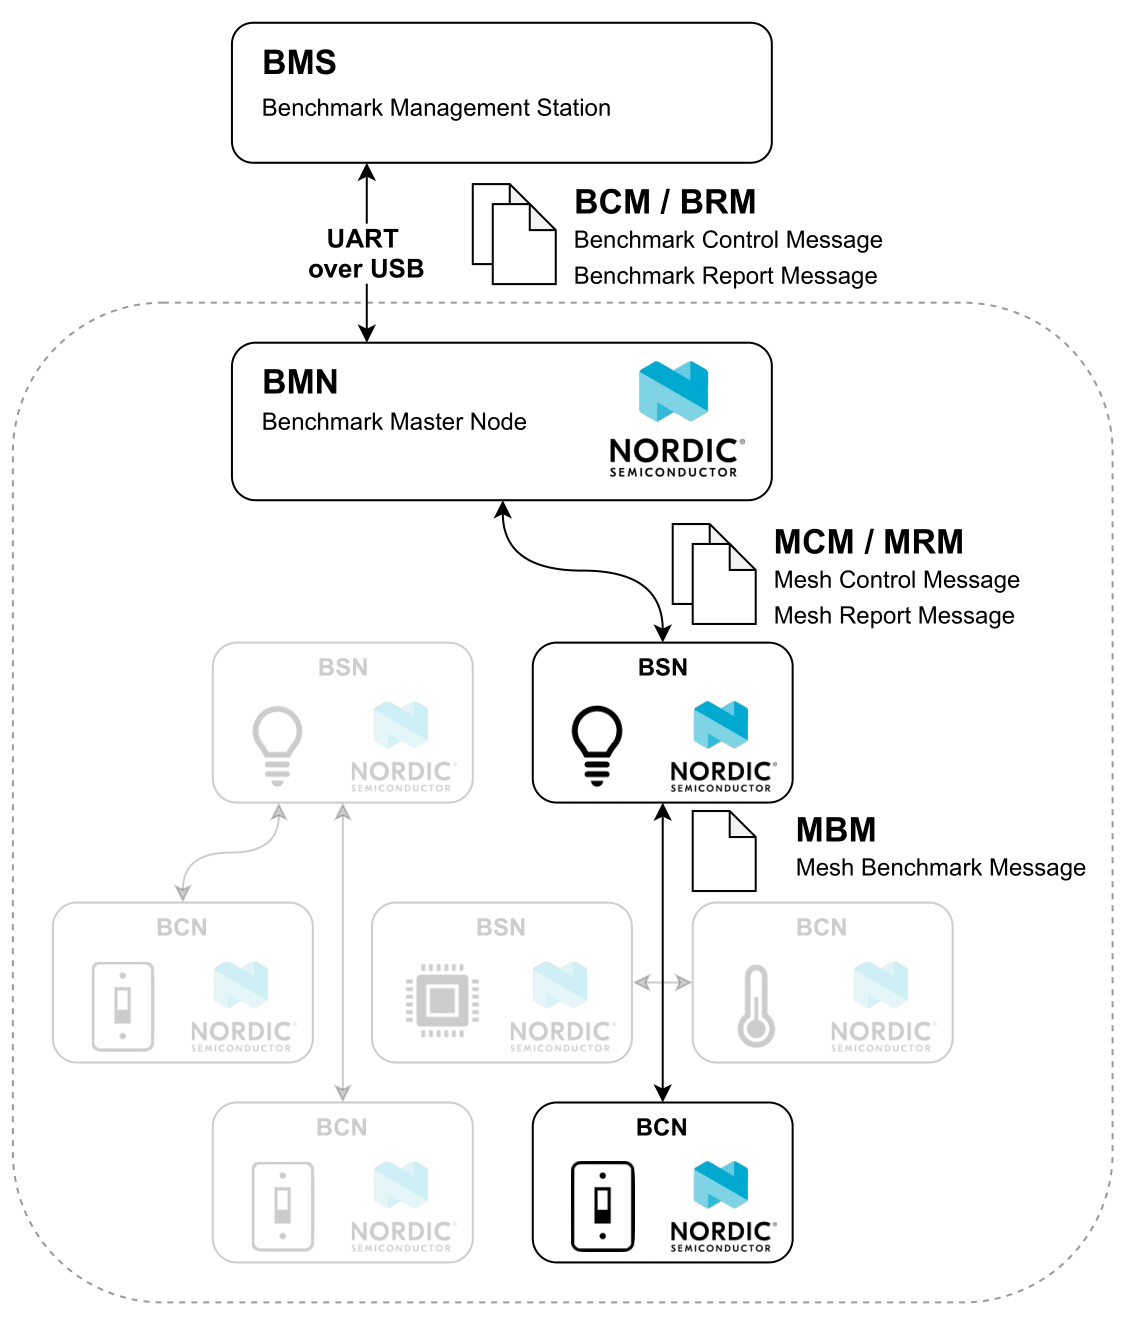
\includegraphics[width=6cm]{graphics/Mesh_Testkonzeptschema.png}
	\caption{Konzeptschema Testablauf}
	\label{fig:KonzeptschemaTestablauf}
\end{figure}


\subsection{Messaufbau}
Unterschiedliche Testumgebungen sollen die Benchmarks und schlussendlich den Vergleich der 3 Mesh Protokolle aussagekräftiger machen. Nachfolgende Umgebungen mit den entsprechenden Eigenschaften sollen getestet werden. Die Abbildungen zu den Testumgebungen zeigen jeweils die Platzierung der Nodes sowie deren Funktion und Gruppen Zugehörigkeit. Die Farbe Grün identifiziert den Node als Client Node während Blau für einen Server Nodes steht. Die Nummerierung zeigt welcher Node zu welcher Adressgruppe gehört. Ein Client Node in Gruppe 1 sendet jeweils Nachrichten zu allen Server Nodes in der selben Gruppe.

\paragraph{Labor}
Der Laboraufbau ist ein Extremtest welcher die Leistungsgrenzen der Protokollstacks ausloten soll. Dabei werden die Nodes auf einem Raster gemäss Abbildung \ref{fig:TestaufbauLabor} angeordnet. Die genauen Abmessungen sind der Abbildung zu entnehmen.

\begin{itemize}
	\item Testaufbau unter Laborbedingungen auf engstem Raum.
	\item Ausgeglichene Anzahl Sensoren und Aktoren.
	\item Sehr Hohe Node-Dichte.
	\item Geringe bis keine Störbeeinflussung durch die Umgebung zu erwarten.
	\item Die Mesh-Beziehungen werden künstlich bestimmt sodass einfache P2P Verbindungen mit oder ohne Hop entstehen.
\end{itemize}

\begin{figure}[h]
	\centering
	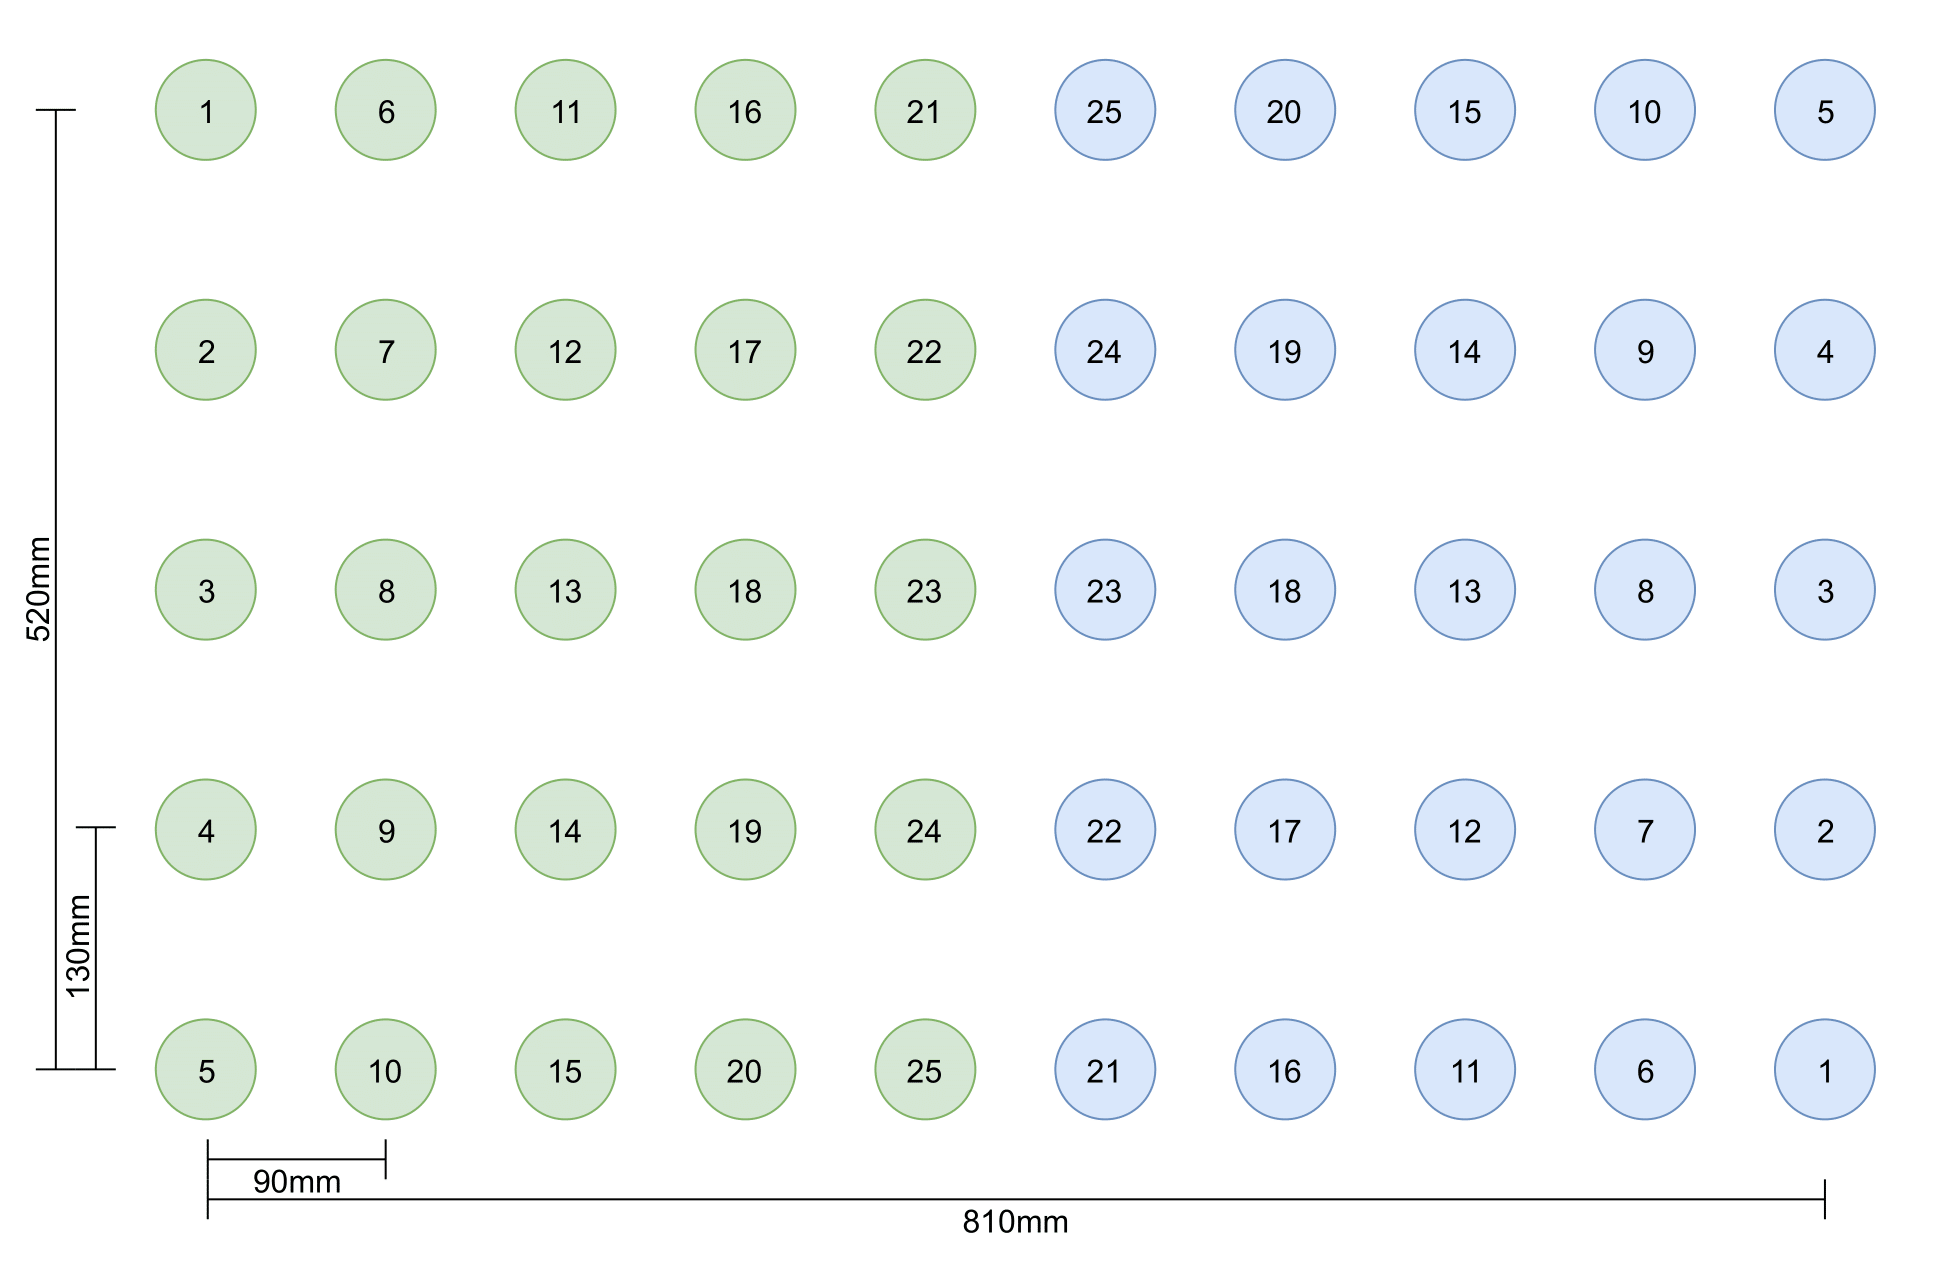
\includegraphics[width=6cm]{graphics/Testaufbau_Labor.png}
	\caption{Testaufbau Labor}
	\label{fig:TestaufbauLabor}
\end{figure}

\paragraph{Einfamilienhaus}
Die Testgeräte werden in einem Einfamilienhaus installiert und repräsentieren damit eine flächendeckende Heim-Automatisierung. Folgende Eingenschaften soll diese Messung abdecken:
\begin{itemize}
	\item Einfamilienhaus über mehrere Etagen.
	\item Anzahl Sensoren und Aktoren vergleichbar gross.
	\item Node-Dichte relativ gering.
	\item Kleine Beeinflussung durch Nachbarsysteme sind zu erwarten.
\end{itemize}

Die Abbildung \ref{fig:TestaufbauHaus} zeigt den Schnitt des Einfamilienhauses in welchem der Benchmark durchgeführt wurde.
\begin{figure}[h]
	\centering
	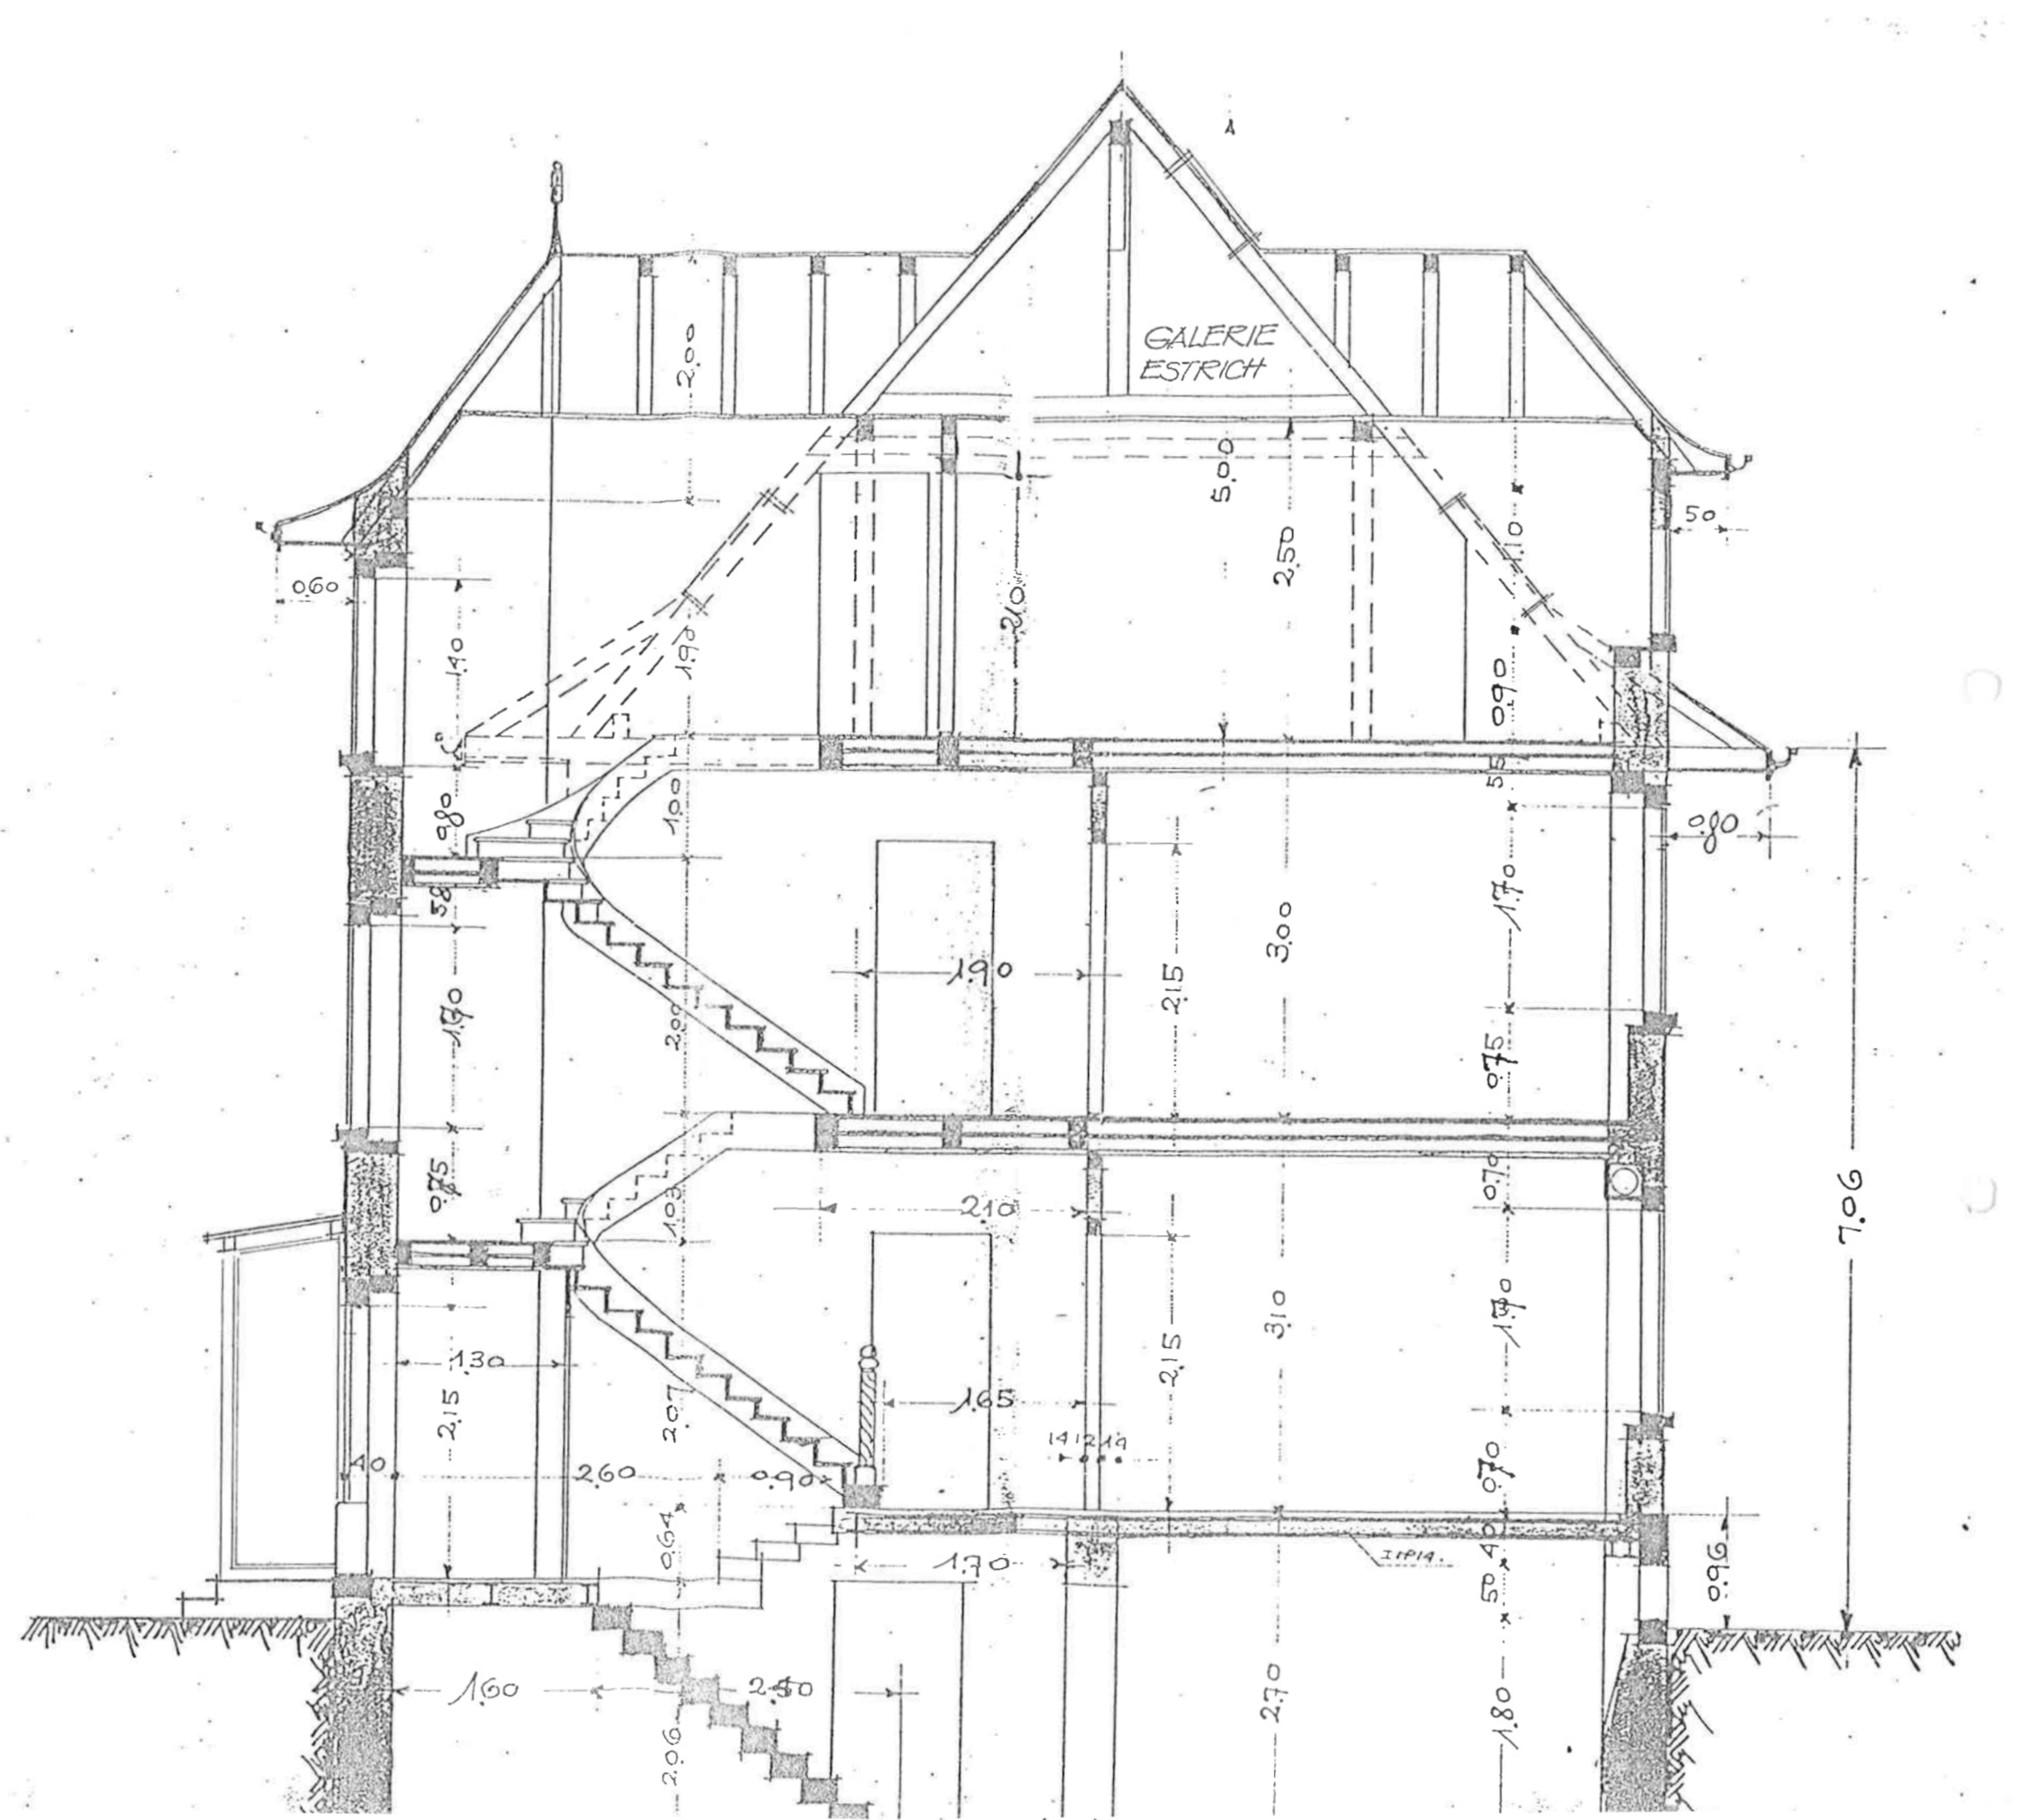
\includegraphics[width=6cm]{graphics/Testaufbau_Haus_Schnitt.png}
	\caption{Testaufbau Haus}
	\label{fig:TestaufbauHaus}
\end{figure}

\paragraph{Wohnung}
Ebenfalls als Heim-Automatisierung gedacht werden die Messungen in einer Wohnung durchgeführt.
\begin{itemize}
	\item Wohnung über eine Etage in einem Mehrfamilienhaus
	\item Anzahl Sensoren und Aktoren vergleichbar gross.
	\item Node-Dichte höher als im Haus.
	\item Mögliche Störeinflüsse durch andere Systeme von Nachbarn sind zu erwarten.
\end{itemize}

Bei der Wohnung handelt es sich um eine 3.5 Zimmer Wohnung mit einer Wohnfläche von 122 Quadratmetern. Die genauen Abmessungen sowie die Platzierung der Nodes ist in Abbildung \ref{fig:TestaufbauWohnung} zu sehen.
\begin{figure}[h]
	\centering
	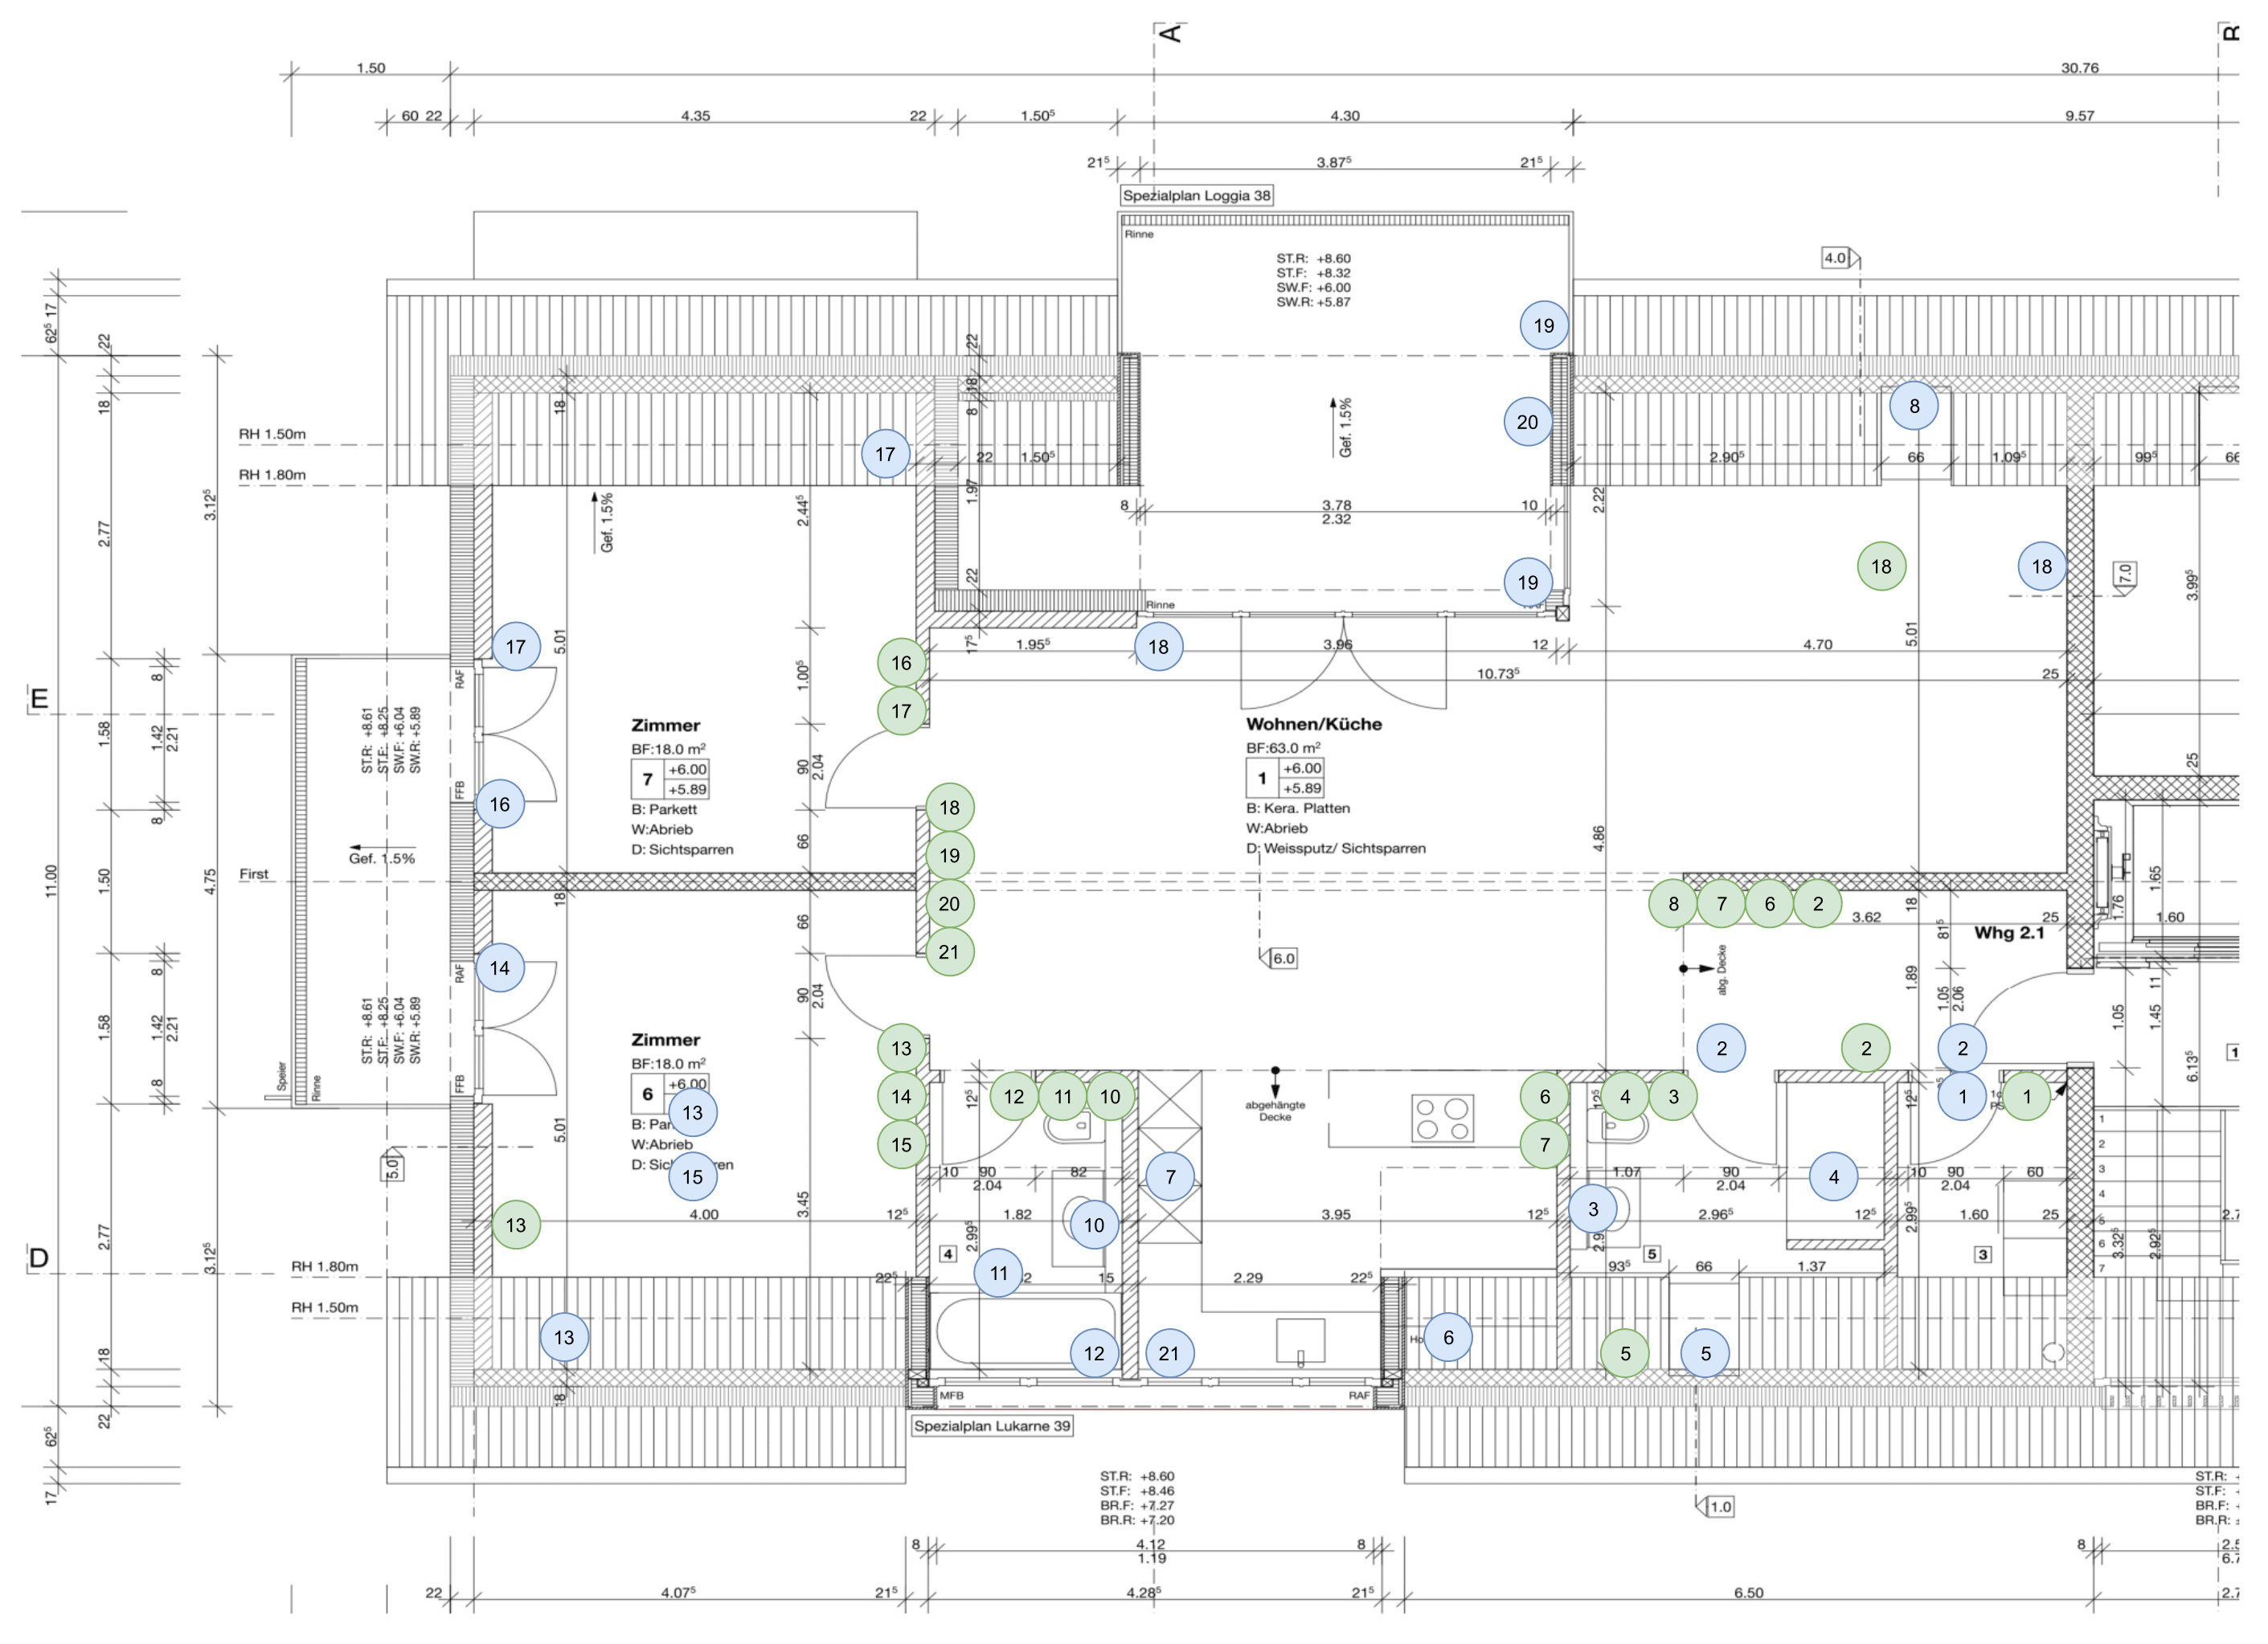
\includegraphics[width=6cm]{graphics/Plan_Wohnung_Cyrill_Nodes_Placement.png}
	\caption{Testaufbau Wohnung}
	\label{fig:TestaufbauWohnung}
\end{figure}


\subsection{Messerwartung}
\todo[inline]{Welche Erwartungen haben wir von den verschiedenen Stacks. (Bluetooth routet nicht daher evtl. langsamer)}

\section{Ergebnisse}
\todo[inline]{Die Ergebnisse sollen hier nach verschiedenen Kriterien dargestellt werden (Anzahl Nodes, Anzahl Hops, usw.)}


\clearpage
\section{Interpretation}\label{sec:Interpretation}

\section{Validierung}
\todo[inline]{Hier soll die Fehlerabschätzung erwähnt werden. Vergleich mit anderen Benchmarks von verschiedenen Organisationen.}
\todo[inline]{Vergleich mit anderen Benchmarks von verschiedenen Organisationen.}

% Document "Appendix":
% ==========================================

\section*{Ergänzende Informationen}
\todo[inline]{Infos die evtl. wichtig sind aber nicht unbedingt in den Kontext gehören}

% Document "References":
% ==========================================
%\bibliography{literature/bibliography}

\end{document}